\subsection{Faraday-Pockels}
\subsubsection{Inspection without applied field}
\paragraph{Diffraction and Bifringence}
The inspection of the experimental setup revealed certain aspects
which we might need to include in our interpretation of the results
later. First we noticed minor diffraction phenomena already between
the exit of the Laser's Gaussian Beam and the beginning of the
Pockelcell, as well as bifringence phenomena which caused difficulties
in focusing the laser.  
\paragraph{Low frequency oscillations} Within the lasersignal 
we observed frequencies about $20 Hz$ with a intensity of $10mV/$diff.
We did not expect these frequencies at first; we will look into it
in the later progress of the experiment.
\subsubsection{Calibration of the Analysator with sawtooth wave}
We did now certain measurements for analyzing the behaviour of a 
certain degree of the analysator.
\newcommand{\picwidth}{0.49\textwidth}

\begin{figure}
    \begin{subfigure}[b]{\picwidth}
        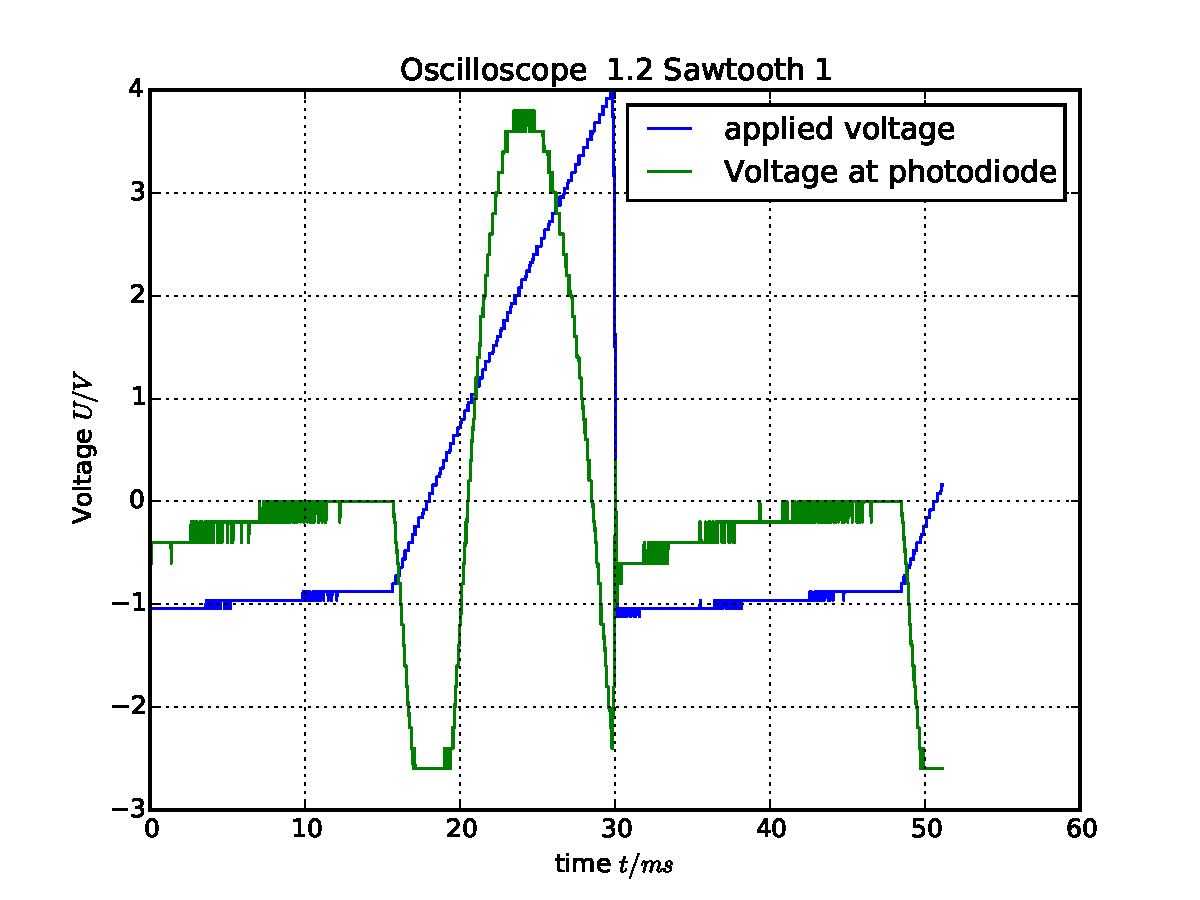
\includegraphics[width=\textwidth]{analysis/figures/12sawtooth1}
        \caption{}
    \end{subfigure}\qquad
    \begin{subfigure}[b]{\picwidth}
        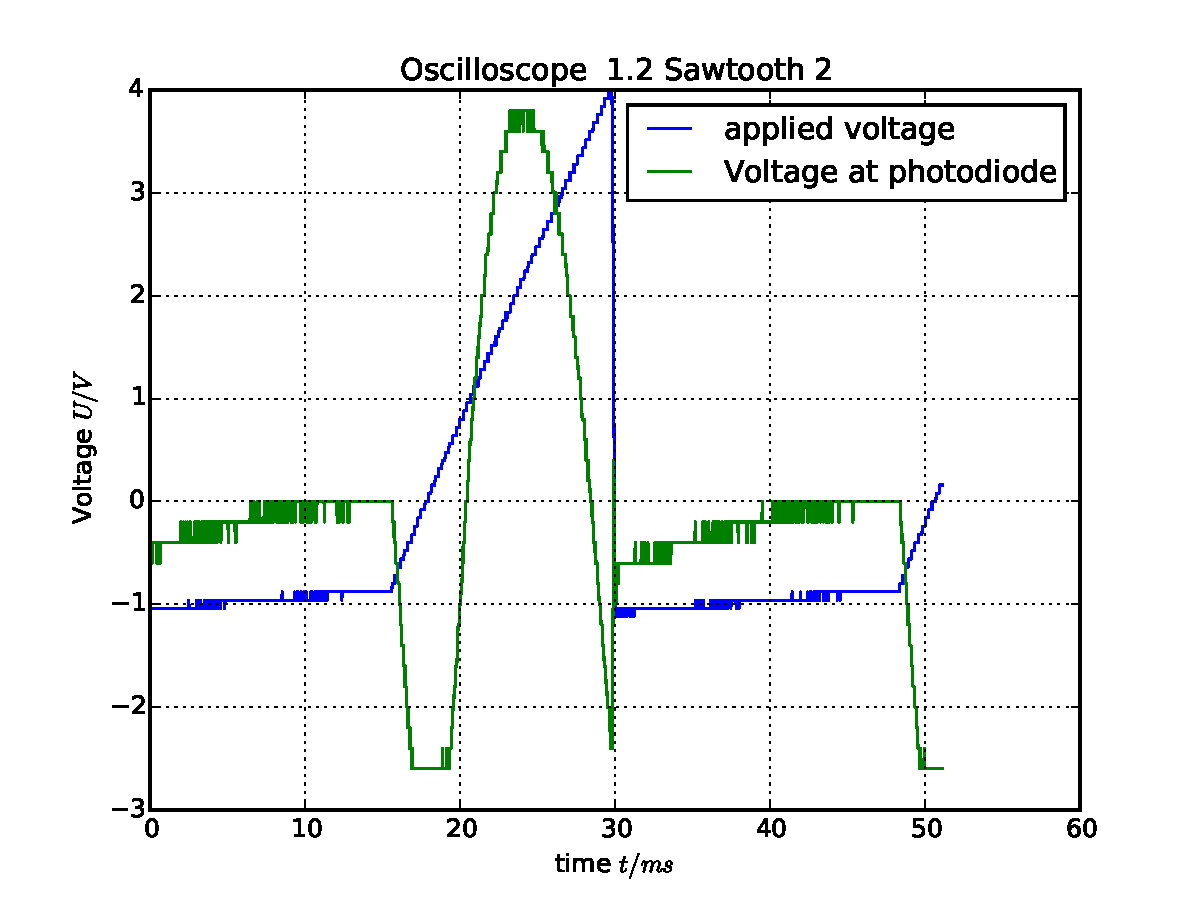
\includegraphics[width=\textwidth]{analysis/figures/12sawtooth2}
        \caption{}
    \end{subfigure}
    \begin{subfigure}[b]{\picwidth}
        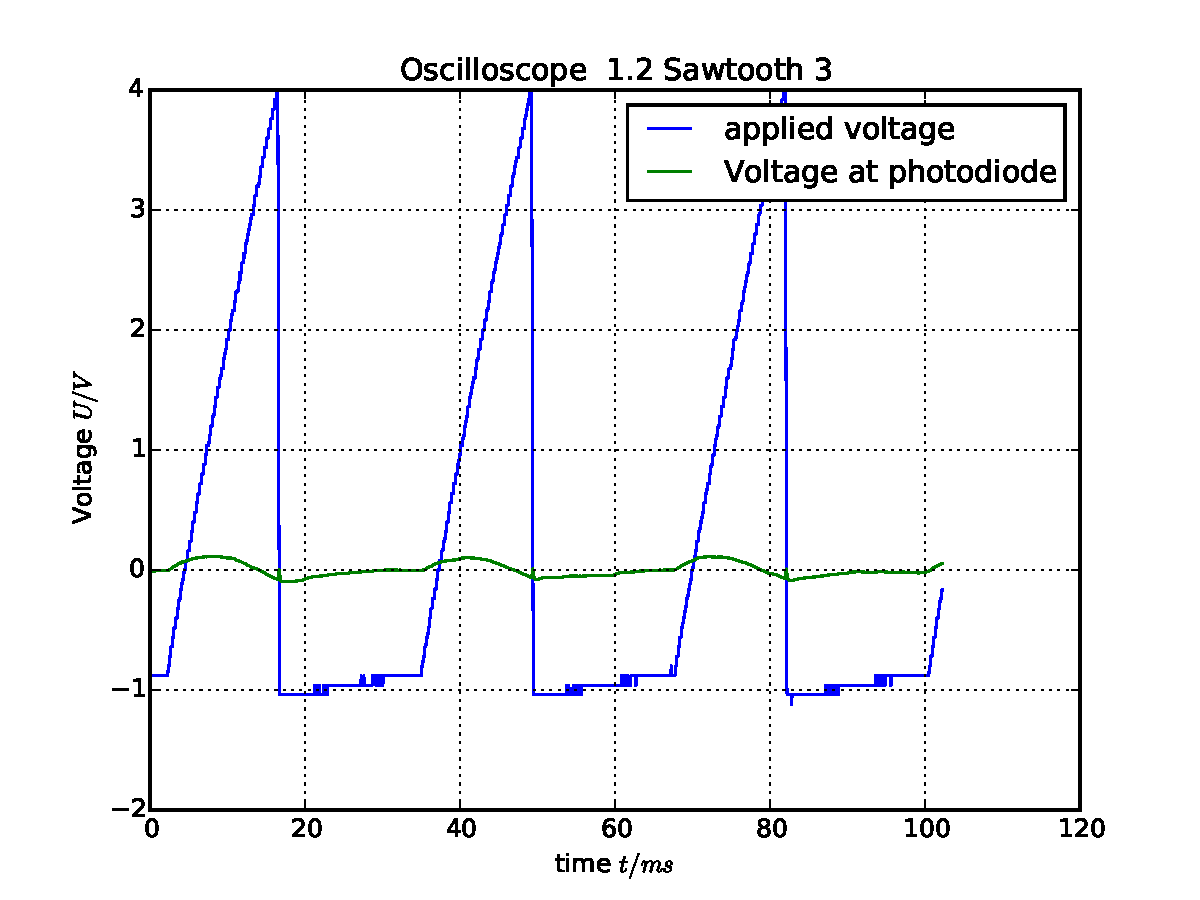
\includegraphics[width=\textwidth]{analysis/figures/12sawtooth3}
        \caption{}
    \end{subfigure}
    \begin{subfigure}[b]{\picwidth}
        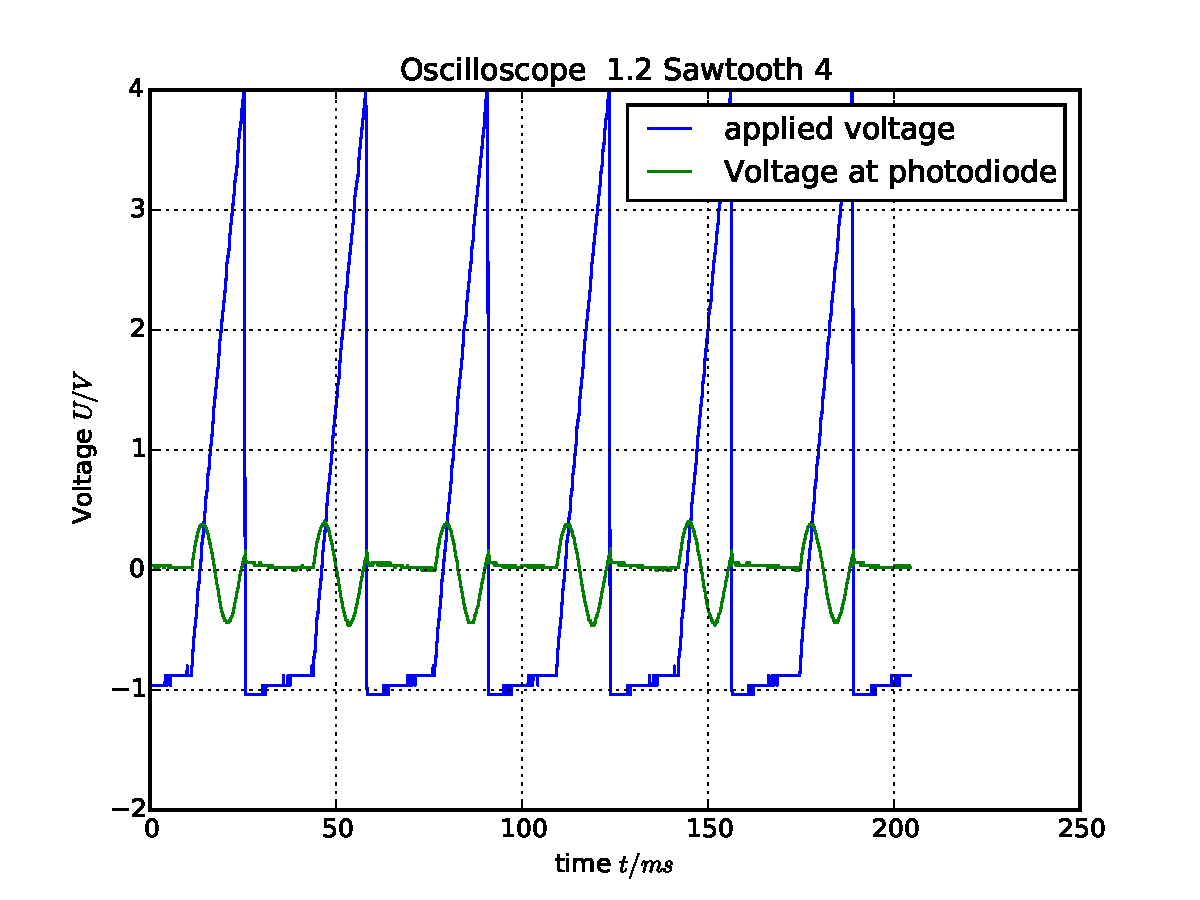
\includegraphics[width=\textwidth]{analysis/figures/12sawtooth4}
        \caption{}
    \end{subfigure}
    \caption{These were the first measurements with the 
        oscillscope in order to calibrate the Analysator.
        The next measurements will show the result of the 
        final calibration. You can find the same configuration
        with different zoom from (b) to (d).}
    \label{fig:saw1}
\end{figure}
\flushleft
\begin{figure}
    \begin{subfigure}[b]{\picwidth}
        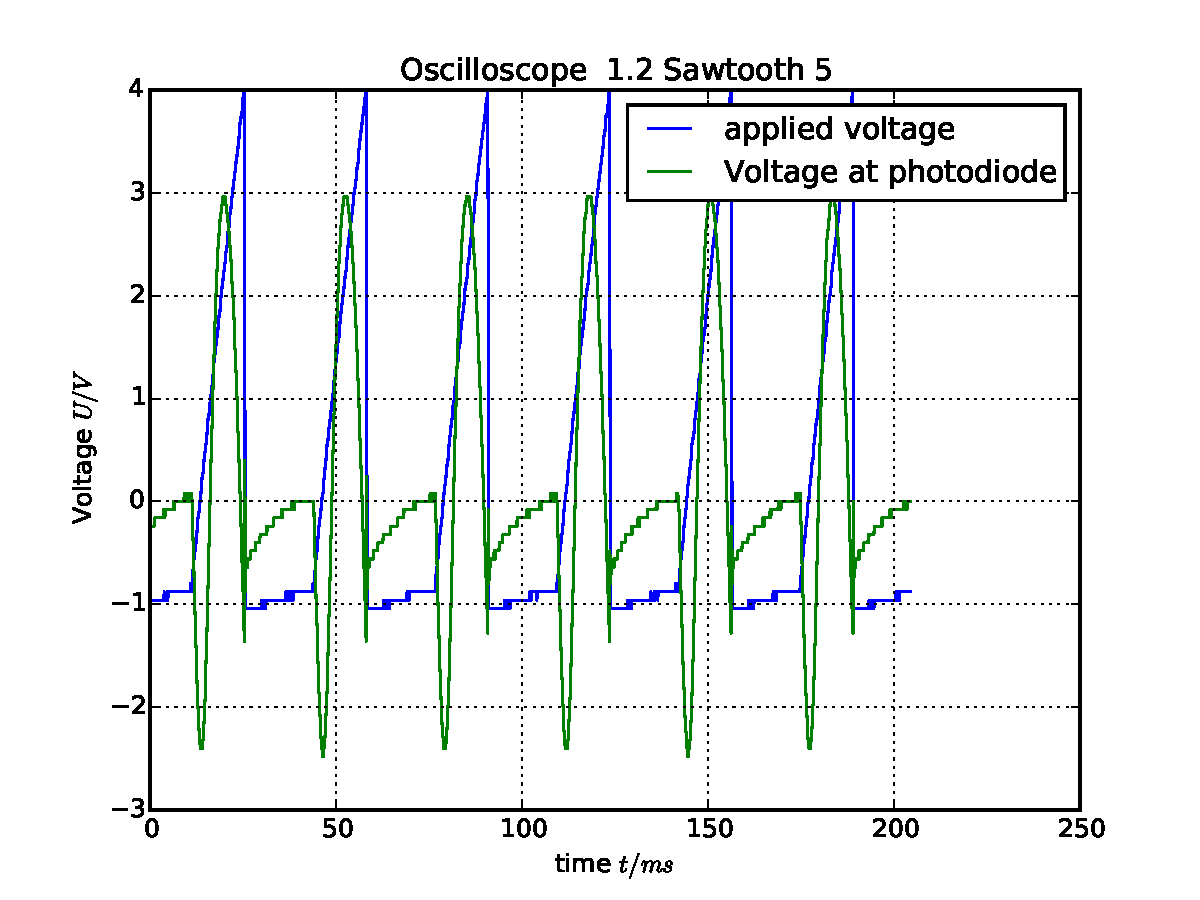
\includegraphics[width=\textwidth]{analysis/figures/12sawtooth5}
        \caption{}
    \end{subfigure}\qquad
    \begin{subfigure}[b]{\picwidth}
        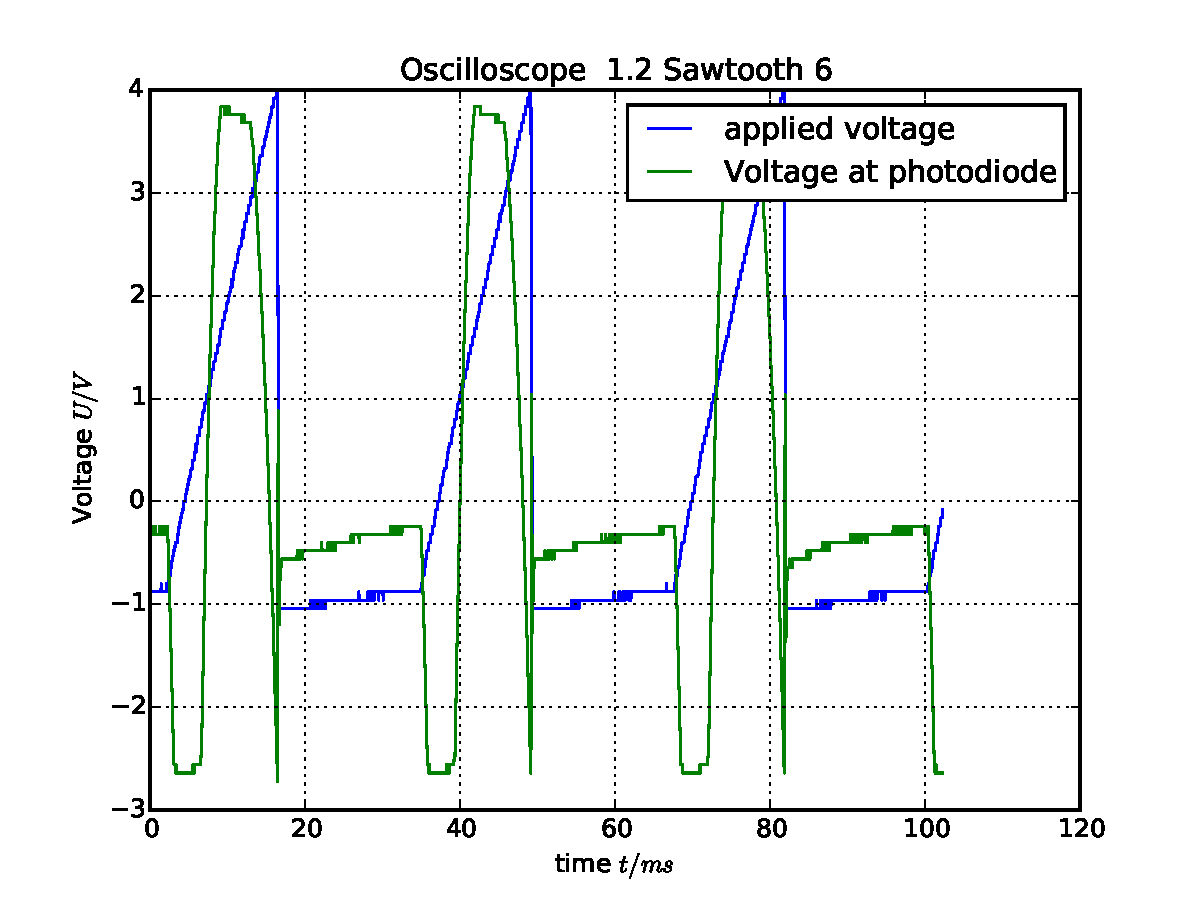
\includegraphics[width=\textwidth]{analysis/figures/12sawtooth6}
        \caption{}
    \end{subfigure}
    \begin{subfigure}[b]{\picwidth}
        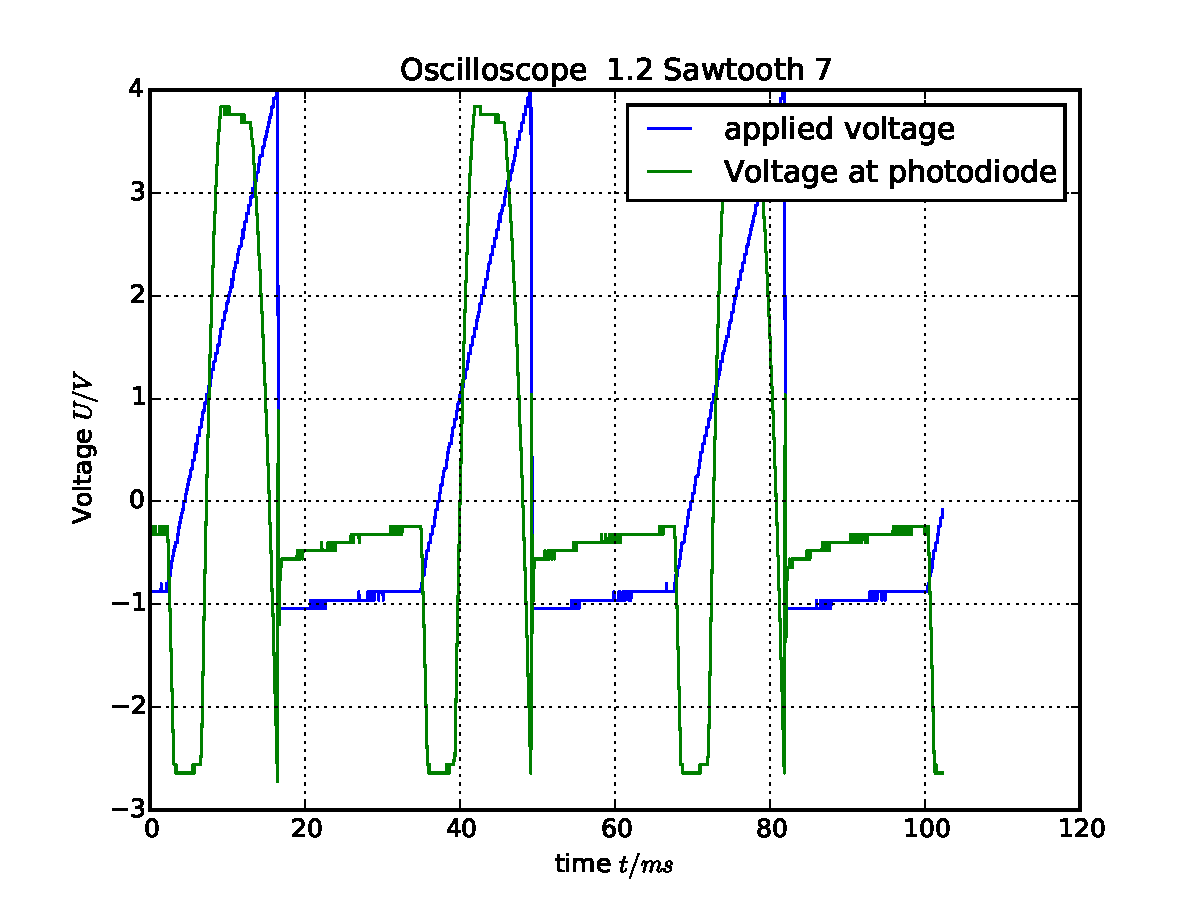
\includegraphics[width=\textwidth]{analysis/figures/12sawtooth7}
        \caption{}
    \end{subfigure}
    \begin{subfigure}[b]{\picwidth}
        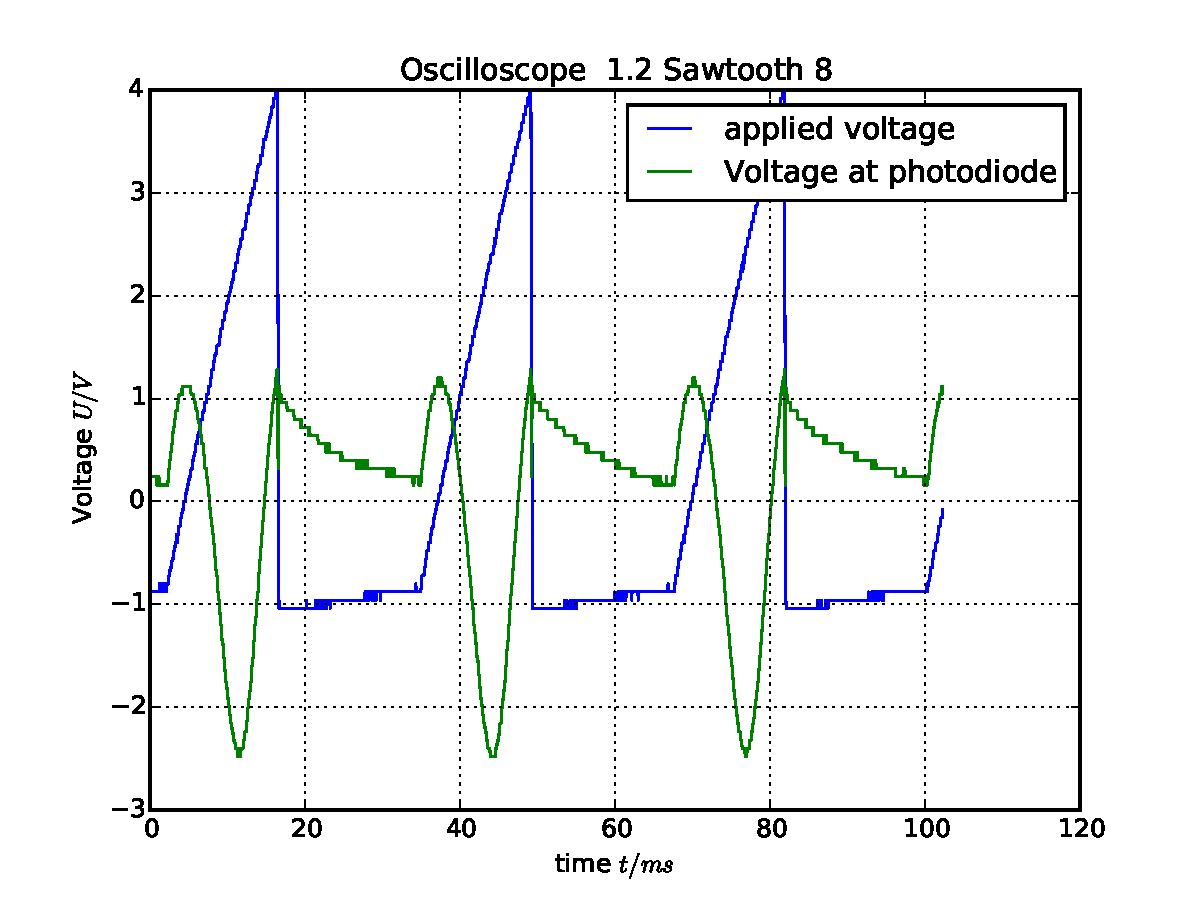
\includegraphics[width=\textwidth]{analysis/figures/12sawtooth8}
        \caption{}
    \end{subfigure}
    \begin{subfigure}[b]{\picwidth}
        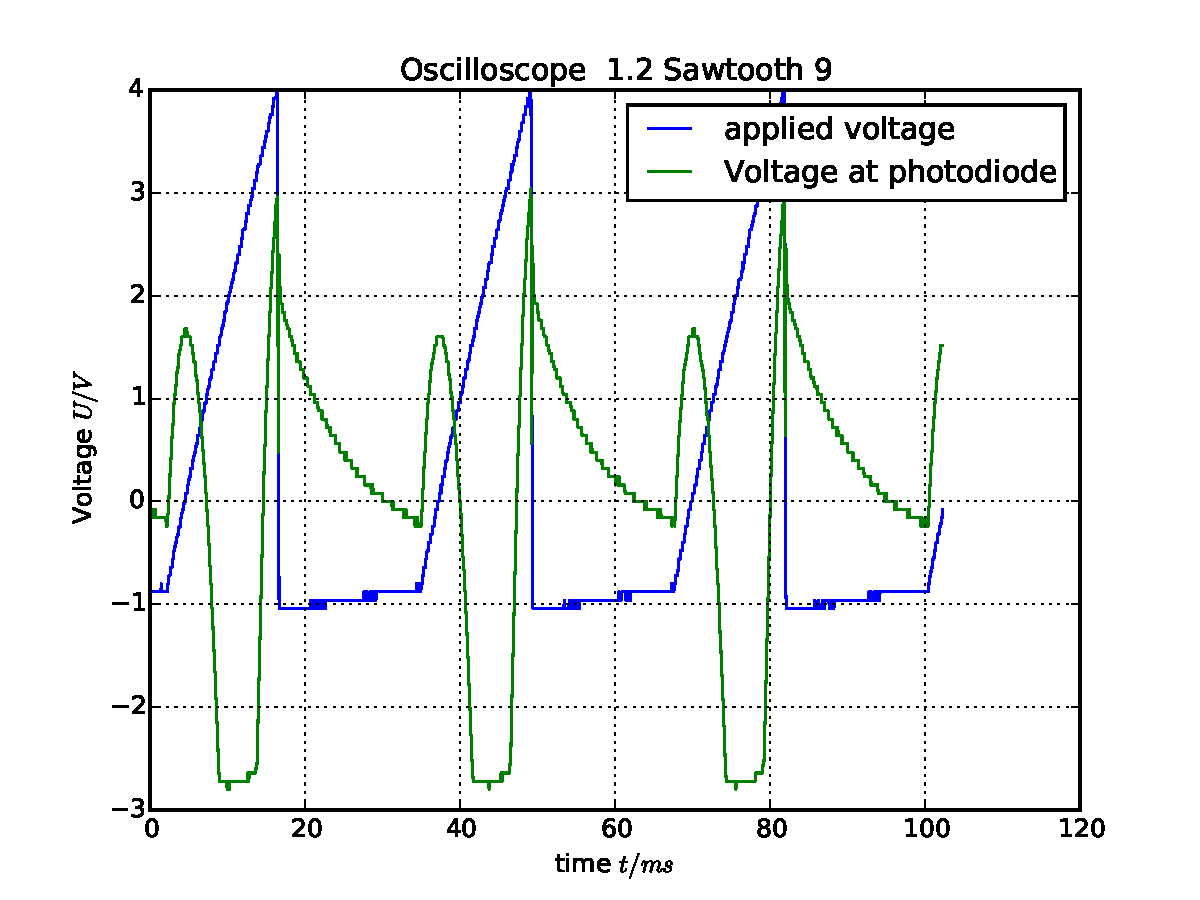
\includegraphics[width=\textwidth]{analysis/figures/12sawtooth9}
        \caption{}
    \end{subfigure}
    \begin{subfigure}[b]{\picwidth}
        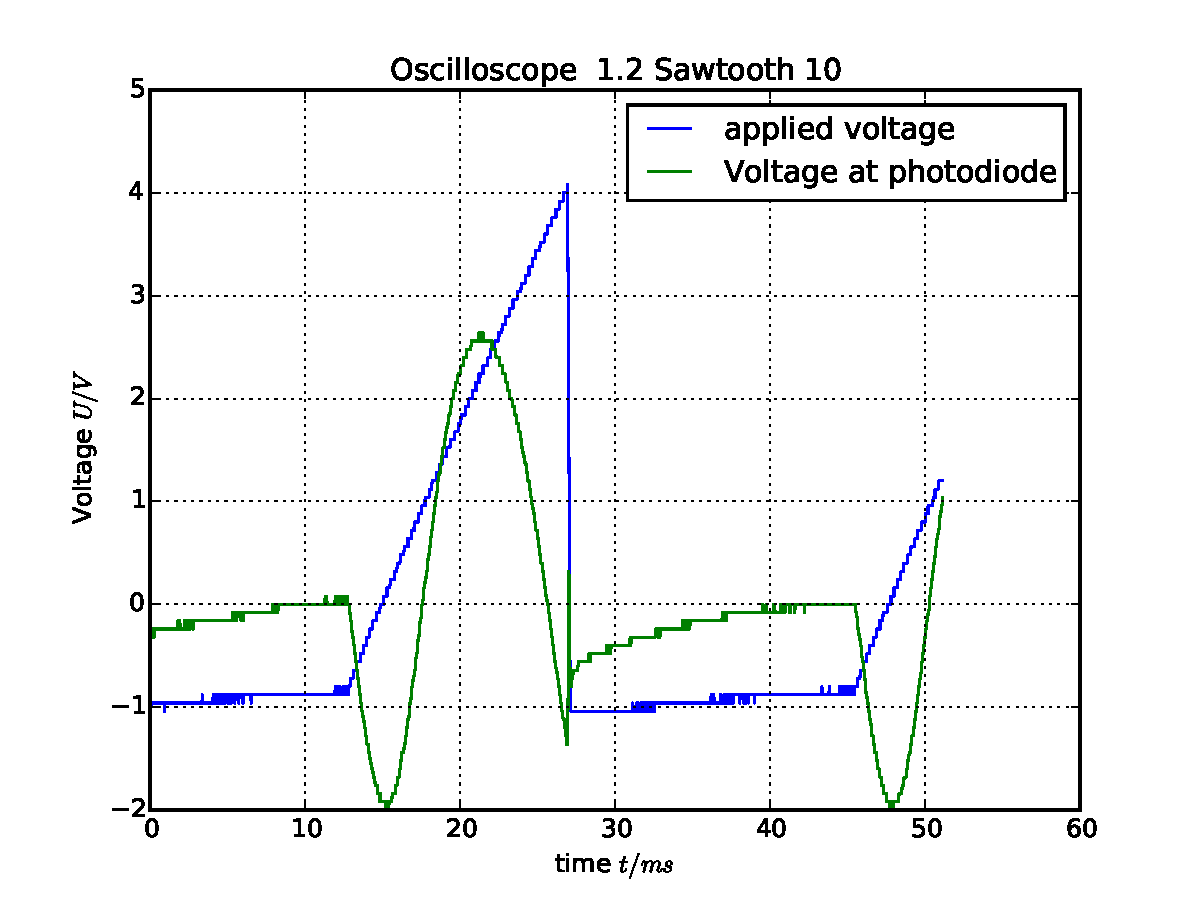
\includegraphics[width=\textwidth]{analysis/figures/12sawtooth10}
        \caption{}
    \end{subfigure}

    \caption{These series of figures show the further 
        attempts to calibrate the analysator. As you can
        notice every figure shows a different degree of the 
        angle and hence the distribution of voltage changes. }
    \label{fig:saw2}
\end{figure}
\flushleft

\begin{figure}
    \begin{subfigure}[b]{\picwidth}
        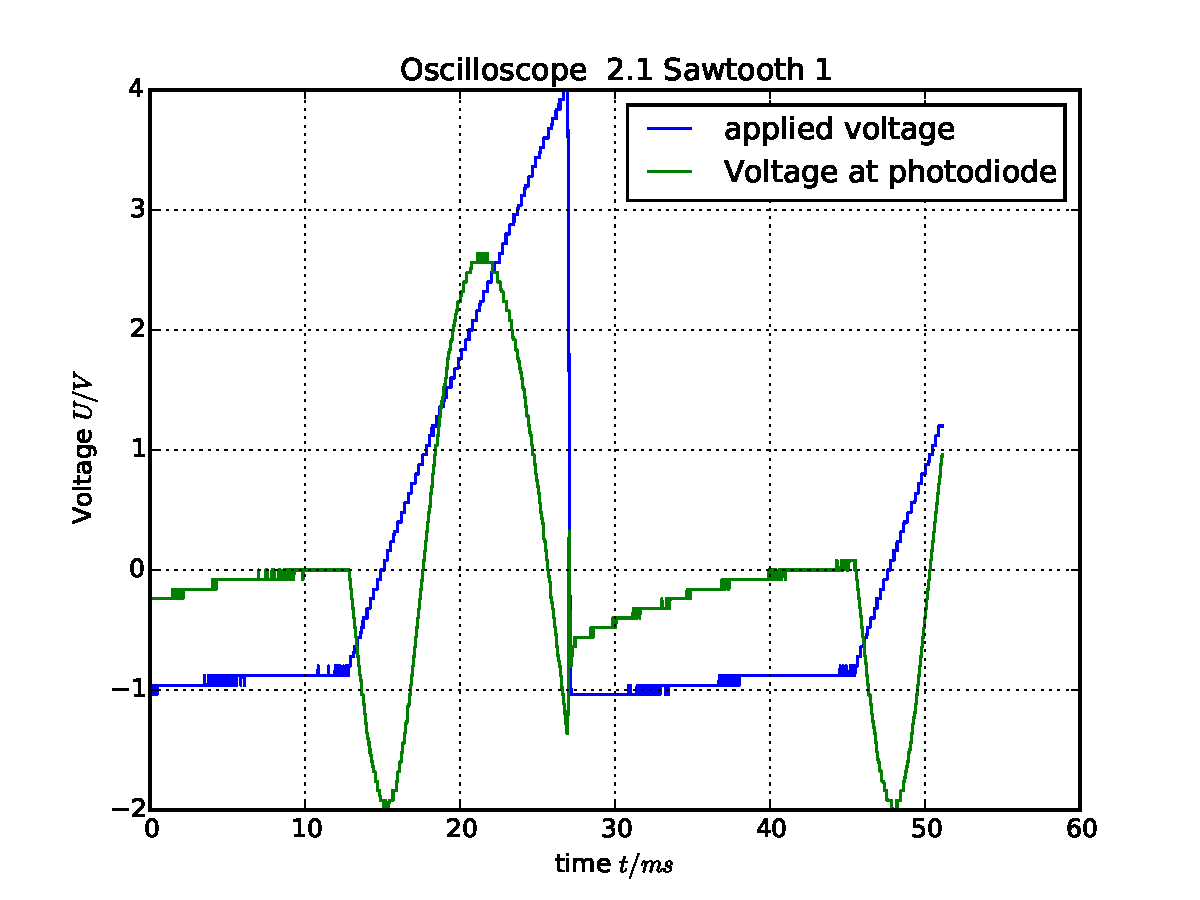
\includegraphics[width=\textwidth]{analysis/figures/21sawtooth1}
        \caption{}
    \end{subfigure}\qquad
    \begin{subfigure}[b]{\picwidth}
        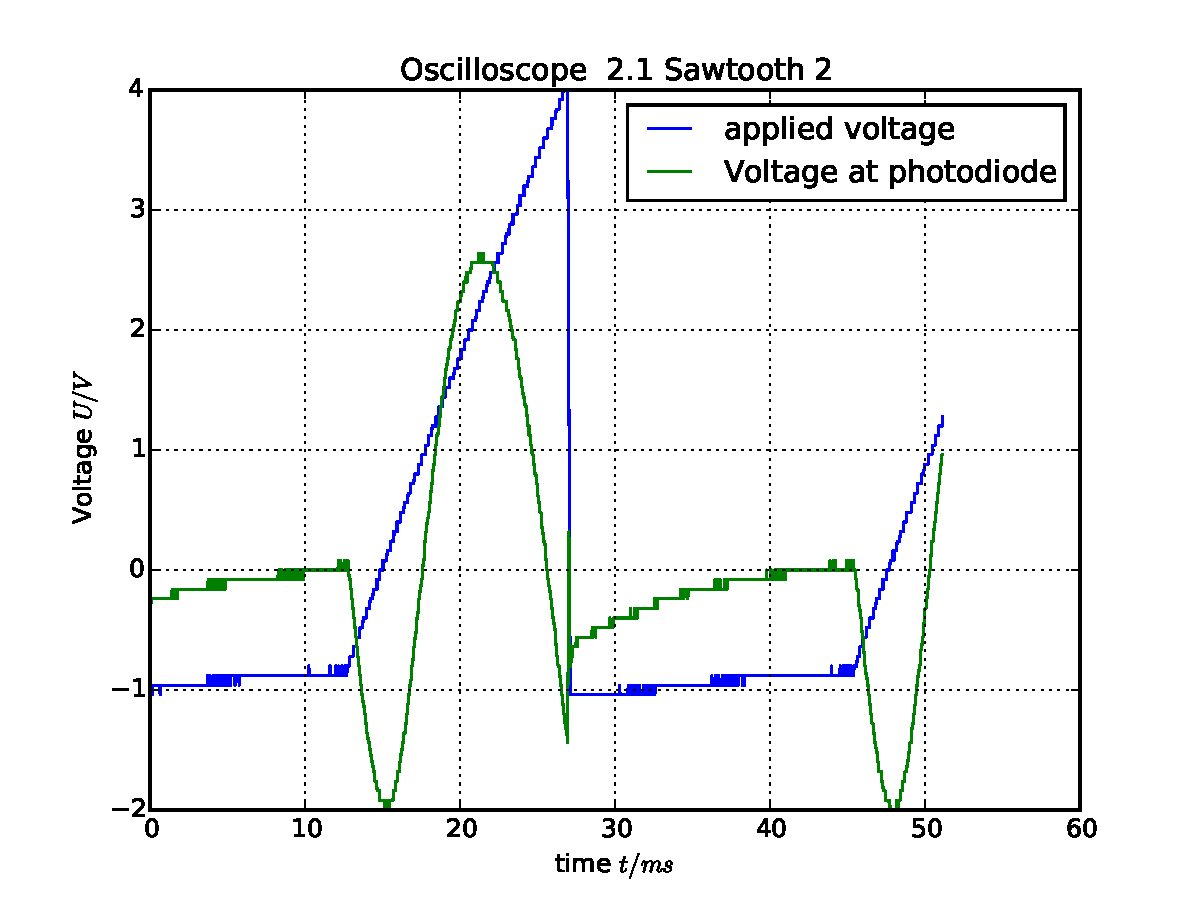
\includegraphics[width=\textwidth]{analysis/figures/21sawtooth2}
        \caption{}
    \end{subfigure}
    \begin{subfigure}[b]{\picwidth}
        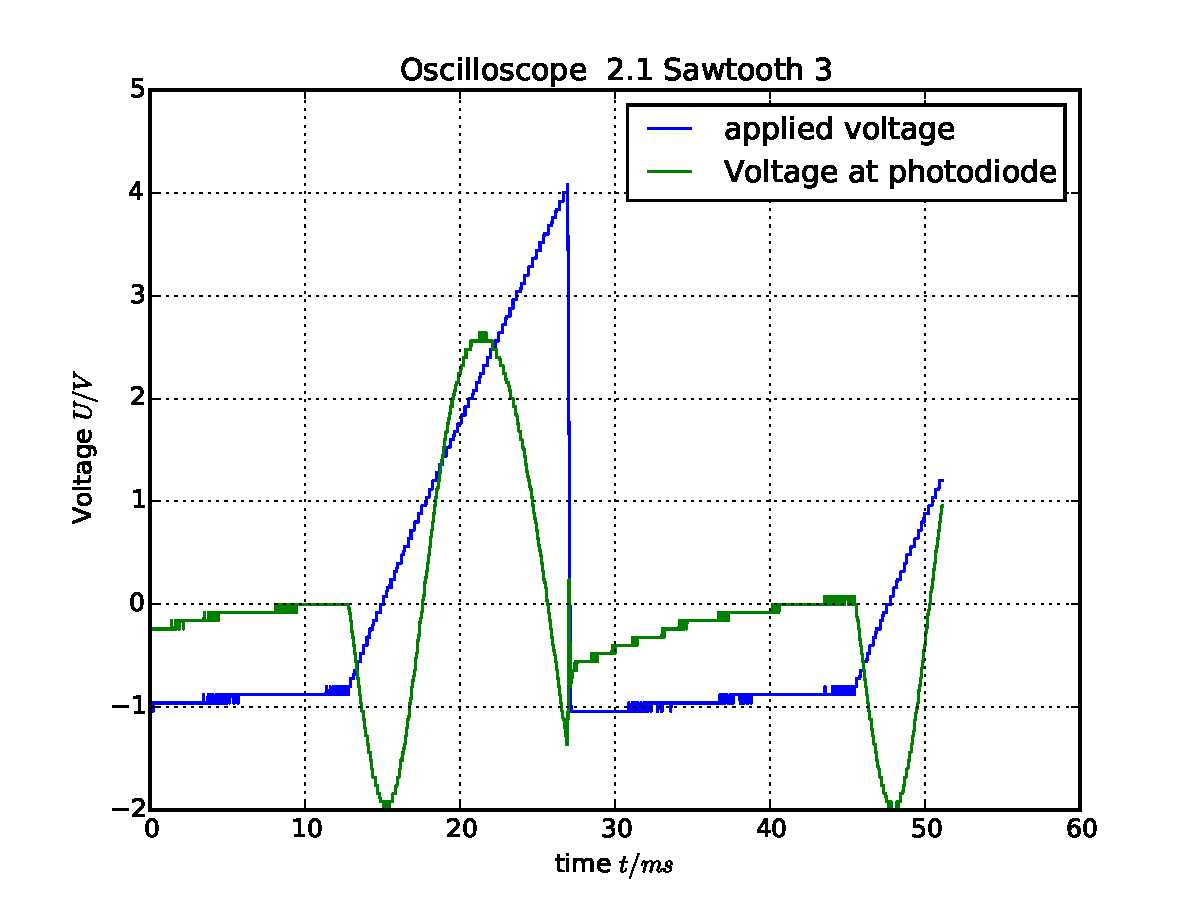
\includegraphics[width=\textwidth]{analysis/figures/21sawtooth3}
        \caption{}
    \end{subfigure}
    \begin{subfigure}[b]{\picwidth}
        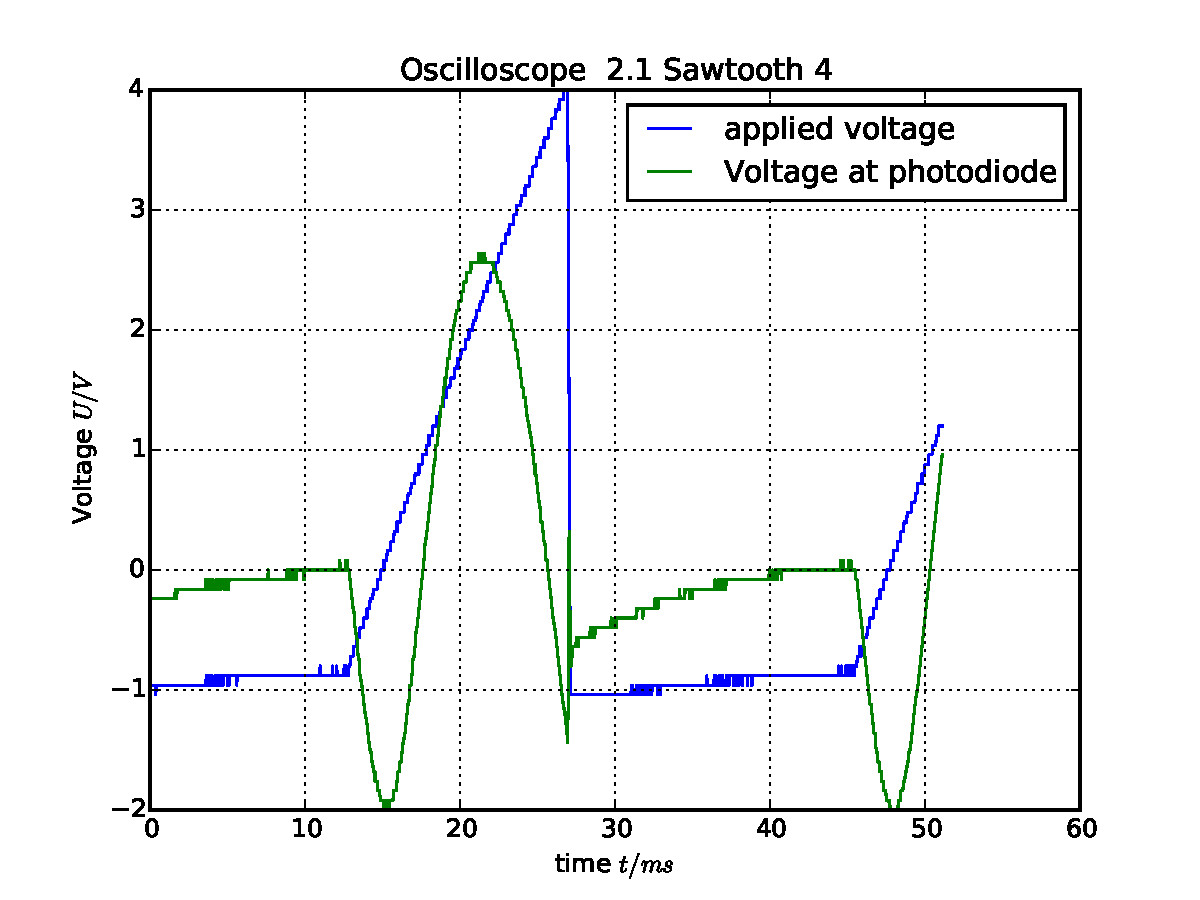
\includegraphics[width=\textwidth]{analysis/figures/21sawtooth4}
        \caption{}
    \end{subfigure}
    \begin{subfigure}[b]{\picwidth}
        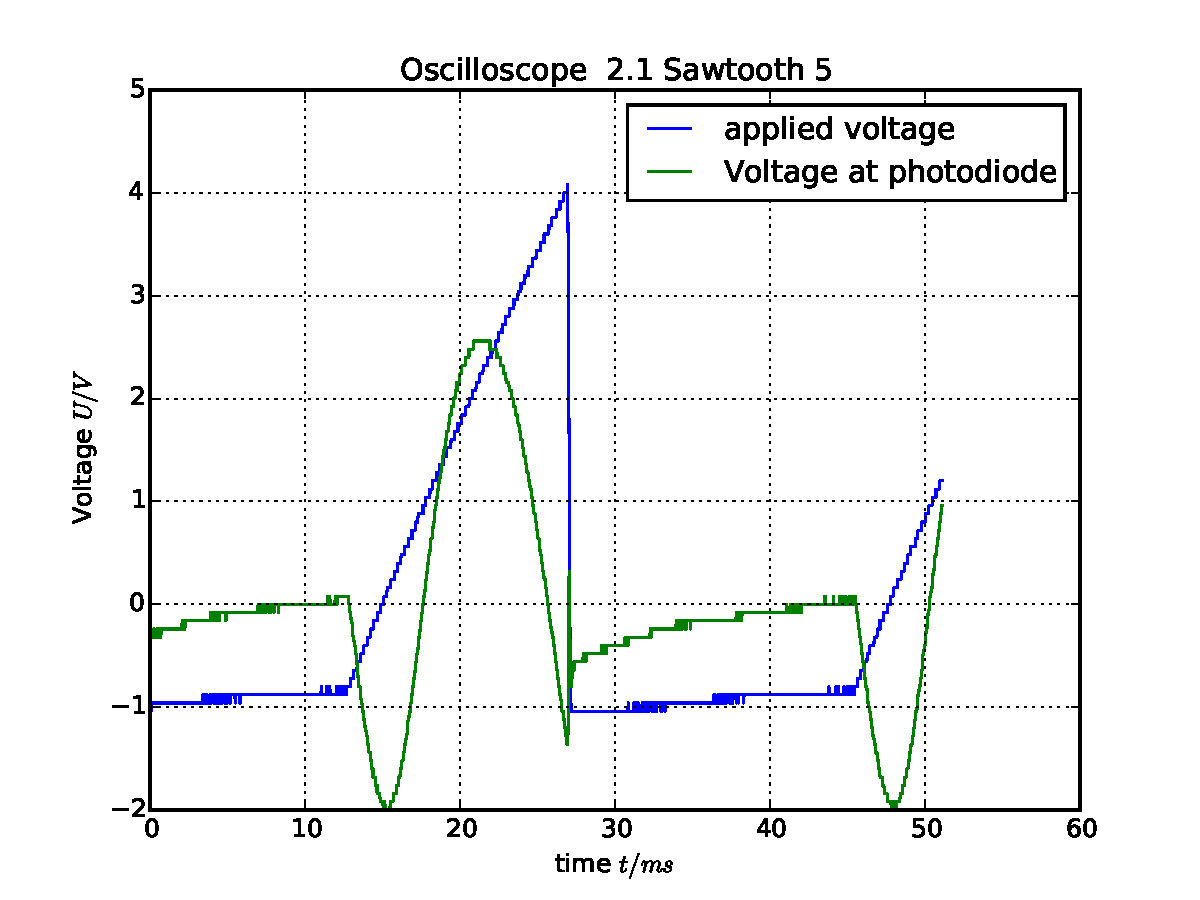
\includegraphics[width=\textwidth]{analysis/figures/21sawtooth5}
        \caption{}
    \end{subfigure}
    \caption{
        This is the final calibration of the analyzer. As you
        can see we did not change the state anymore and all the
        results are in general the same.
        }
    \label{fig:saw3}
\end{figure}
\flushleft
\clearpage
\subsubsection{Sinus-generated Method, without Direct Current}
The Frequency generated was about $f=5.4$ Khz, but it was not stable
but oscillating within $0.1$ Khz. The manipulation of the trigger-
level increased the stability to a acceptable level. 
\begin{figure}
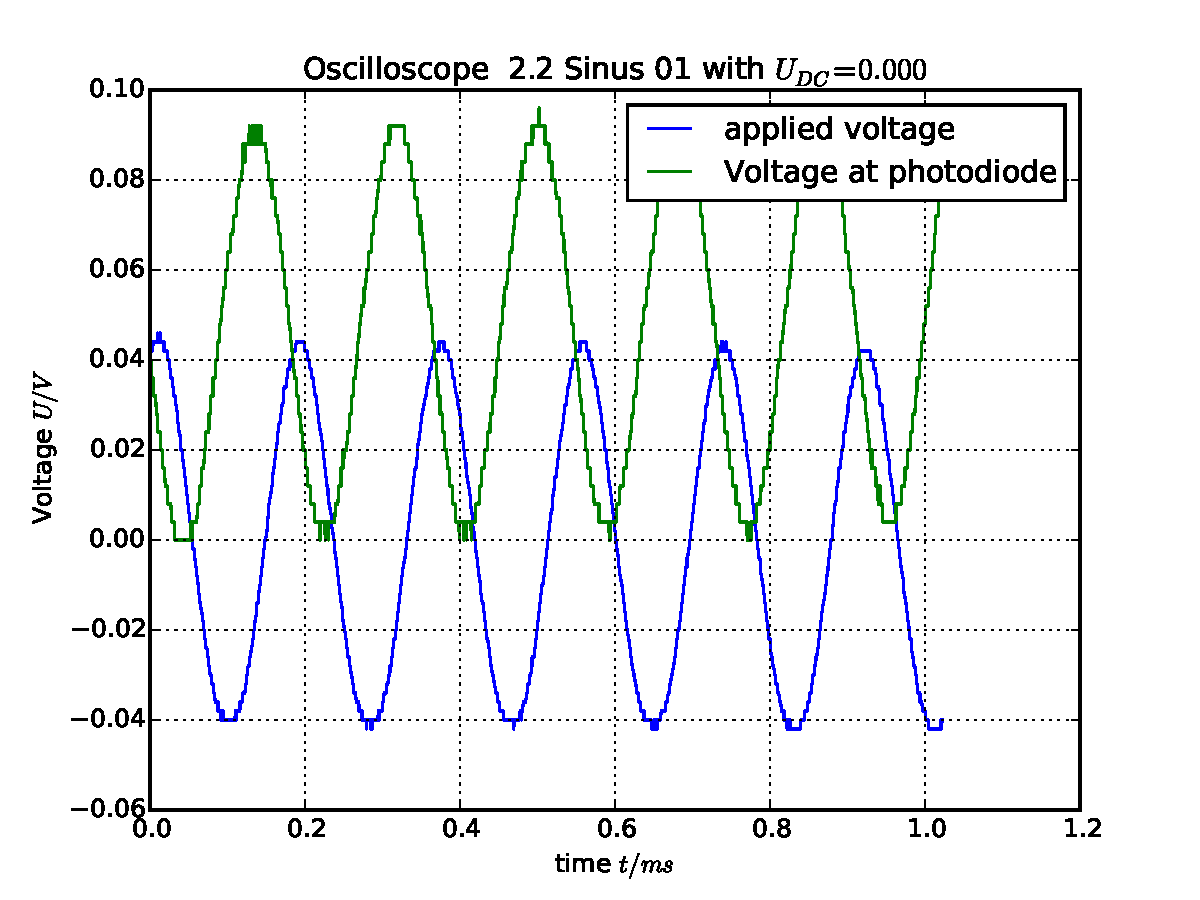
\includegraphics[width=15cm]{analysis/figures/22sinus01}
\end{figure}
\subsubsection{Sinus-generated Method: Applying Direct Current}
Now we will look at the inluence of different parameters on
the received signal, especially the effect of changing the
voltage.
\begin{figure}
    \begin{subfigure}[b]{\picwidth}
        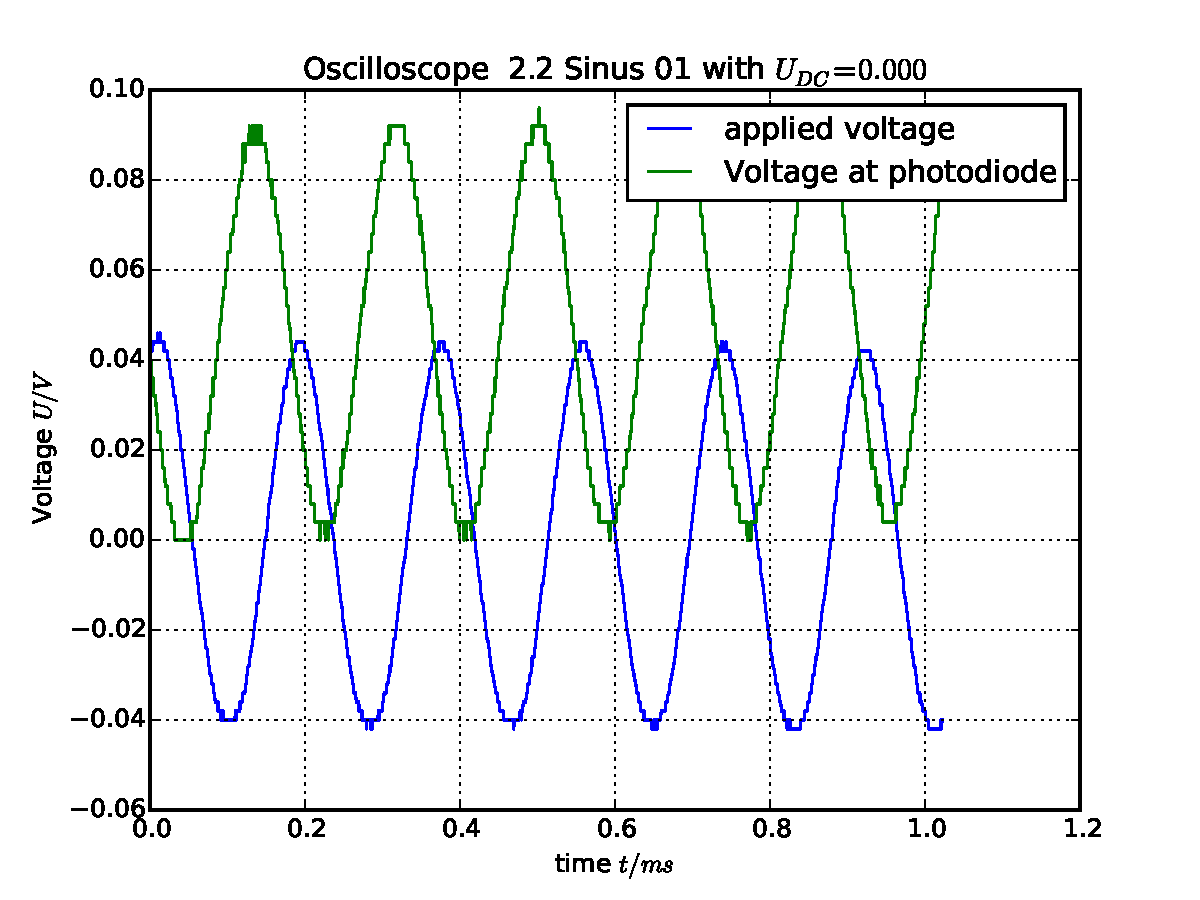
\includegraphics[width=\textwidth]{analysis/figures/22sinus01}
        \caption{}
    \end{subfigure}\qquad
    \begin{subfigure}[b]{\picwidth}
        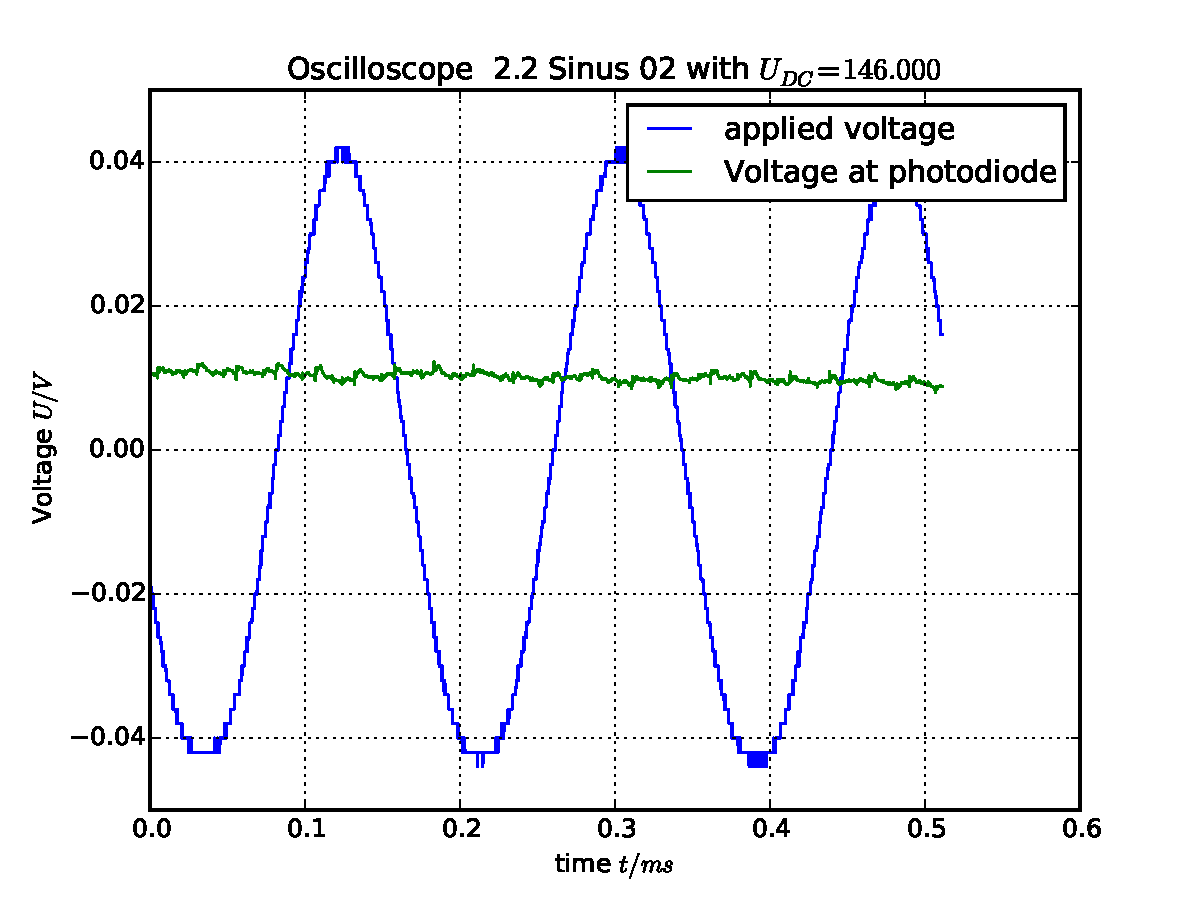
\includegraphics[width=\textwidth]{analysis/figures/22sinus02}
        \caption{}
    \end{subfigure}
    \begin{subfigure}[b]{\picwidth}
        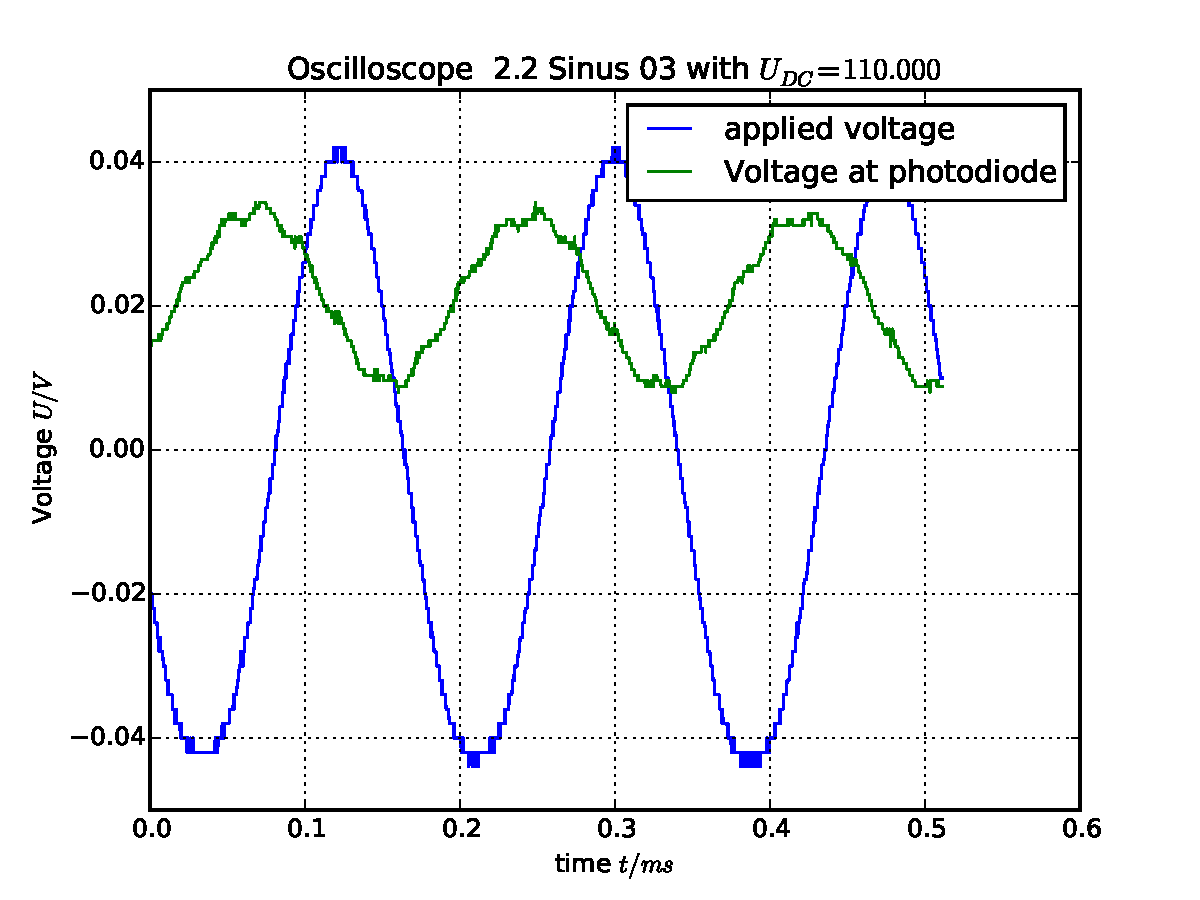
\includegraphics[width=\textwidth]{analysis/figures/22sinus03}
        \caption{}
    \end{subfigure}
    \begin{subfigure}[b]{\picwidth}
        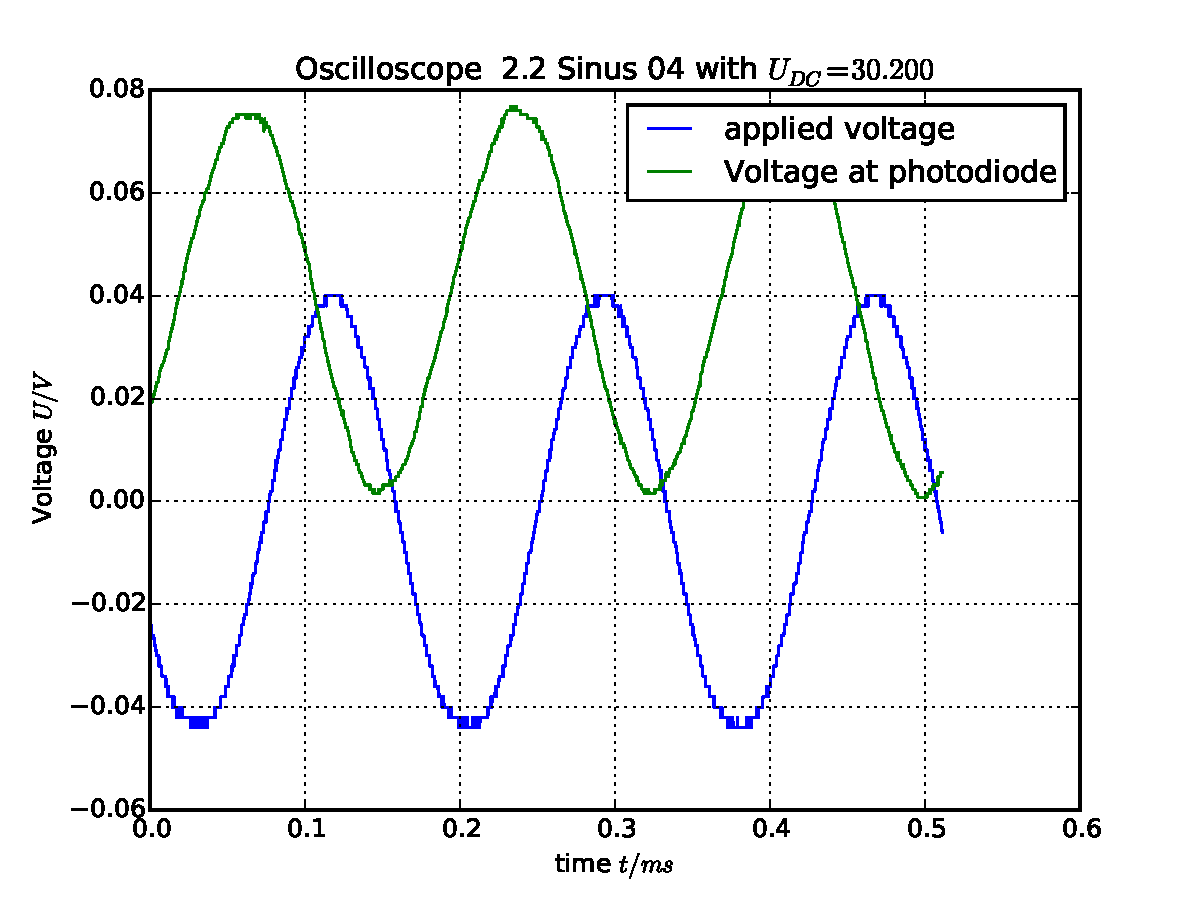
\includegraphics[width=\textwidth]{analysis/figures/22sinus04}
        \caption{}
    \end{subfigure}
    \begin{subfigure}[b]{\picwidth}
        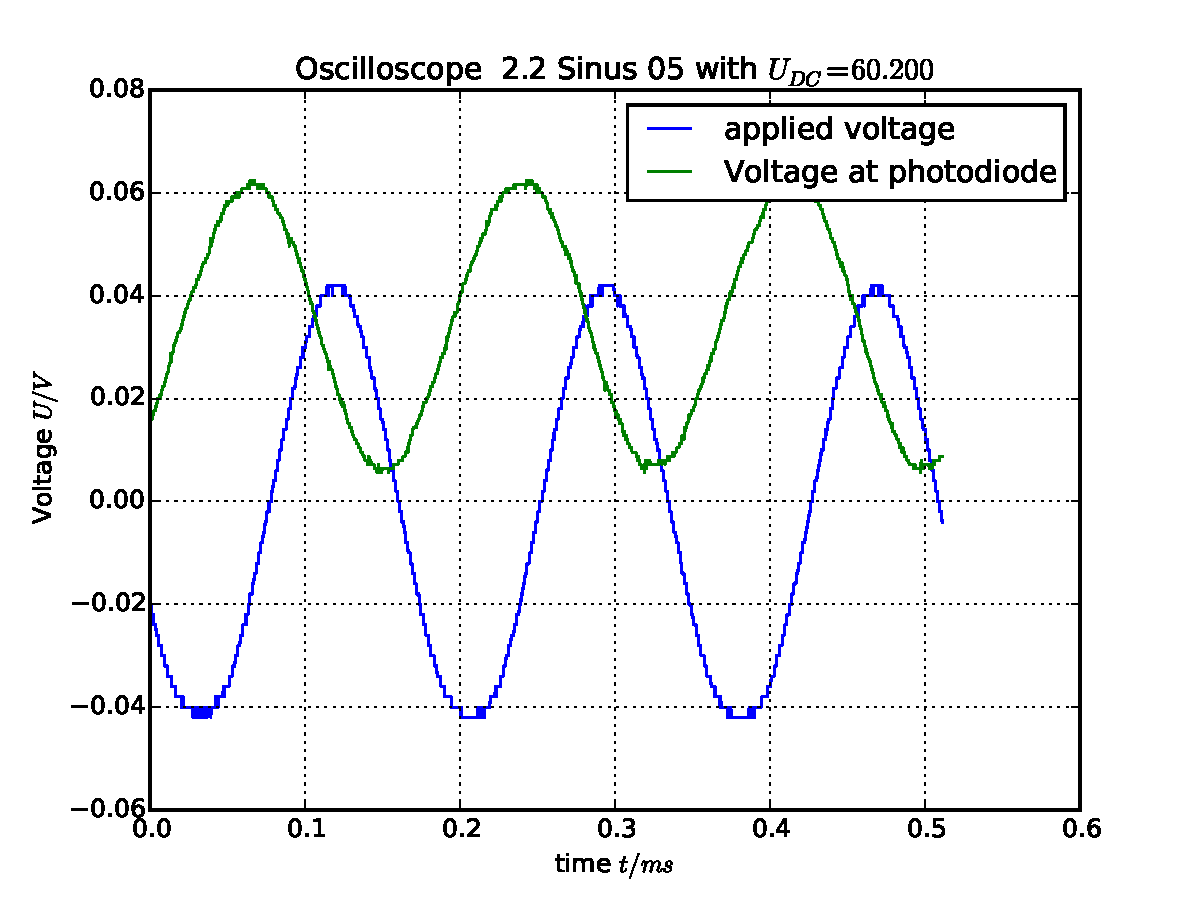
\includegraphics[width=\textwidth]{analysis/figures/22sinus05}
        \caption{}
    \end{subfigure}
    \begin{subfigure}[b]{\picwidth}
        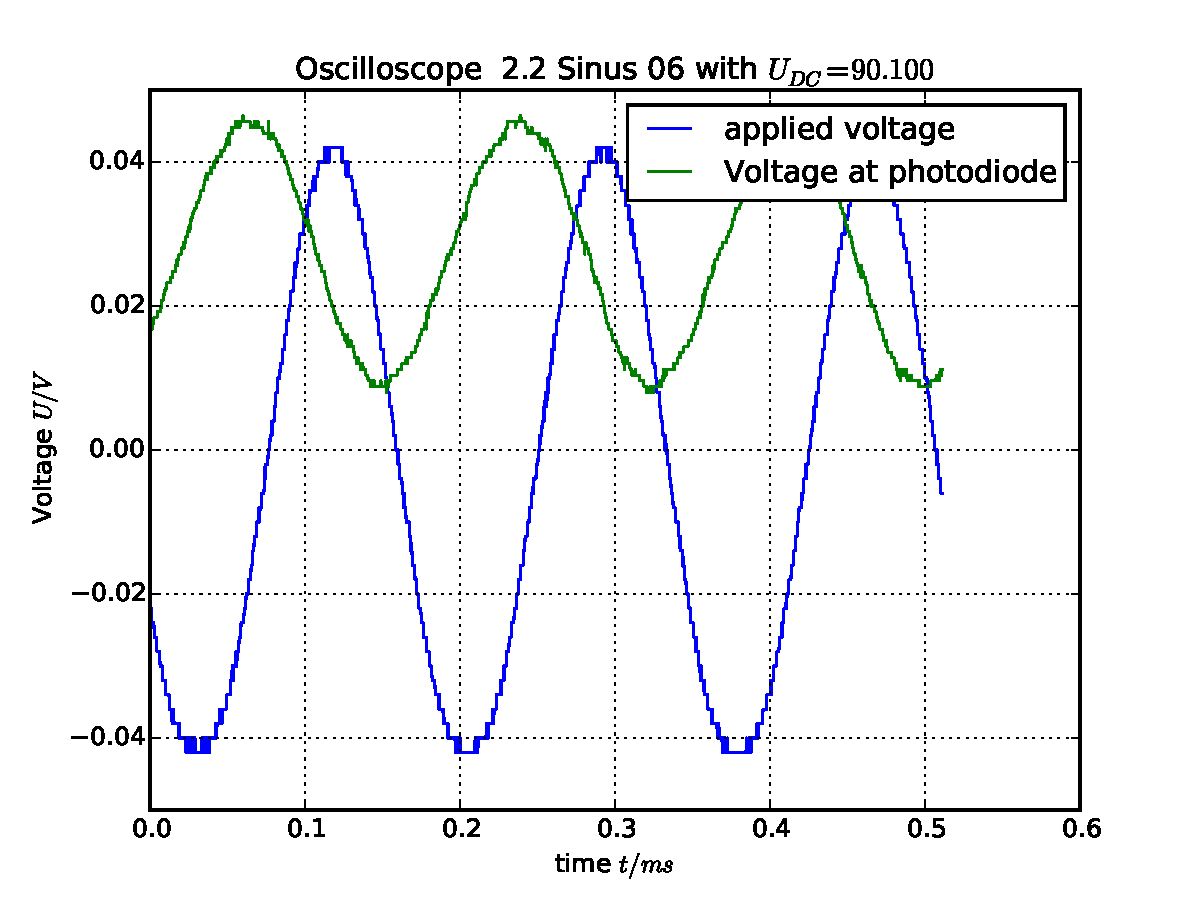
\includegraphics[width=\textwidth]{analysis/figures/22sinus06}
        \caption{}
    \end{subfigure}

    \caption{These series of figures show the impact of
        an applied sinussignal and a Direct Current with
        varying Voltage. In general we do not recognize huge 
        qualitative differences amongst those, but we will look
        later with a more refined analysis to it.}
    \label{fig:sinus1}
\end{figure}
\flushleft


